%% ---------------------------------------------------------------------------
%% This file is part of the "Boost Python" talk.
%%
%% Copyright 2015 by Eugen Wintersberger <eugen.wintersberger@gmail.com>
%%
%% This work is licensed under the Creative Commons
%% Attribution-NonCommercial-ShareAlike 4.0 International License. To view 
%% a copy of this license, visit 
%% http://creativecommons.org/licenses/by-nc-sa/4.0/.
%% ---------------------------------------------------------------------------

\newcommand{\pyobject}{\texttt{object}}
\newcommand{\pylist}{\texttt{list}}
\newcommand{\pytuple}{\texttt{tuple}}
\newcommand{\pydict}{\texttt{dict}}
\newcommand{\pystr}{\texttt{str}}
\newcommand{\pyscope}{\texttt{scope}}
\newcommand{\bpyobject}{\texttt{boost::python::object}}
\newcommand{\bpylist}{\texttt{boost::python::list}}
\newcommand{\bpytuple}{\texttt{boost::python::tuple}}
\newcommand{\bpydict}{\texttt{boost::python::dict}}
\newcommand{\bpystr}{\texttt{boost::python::str}}
\newcommand{\bpyscope}{\texttt{boost::python::scope}}

\section{Creating Python objects}
\begin{frame}{A short overview}
    \texttt{boost::python} provides support for some of the native 
    Python objects
    \vspace{0.1\textheight}
    \begin{itemize}
        \setlength{\itemsep}{0.05\textheight}
        \item \pyobject, \pylist, \pytuple, \pydict
        \item working with strings
        \item \pyscope() - managing the current namespace
    \end{itemize}
\end{frame}

%%%===========================================================================
\begin{frame}[fragile]{Class hierarchy}
    \texttt{boost::python} provides native implementations for 
    \begin{itemize}
        \item lists \bpylist
        \item tuples \bpytuple
        \item dictionaries \bpydict
        \item strings \bpystr
    \end{itemize}
    \vspace{0.025\textheight}
    \begin{center}
        % Graphic for TeX using PGF
% Title: /home/eugen/Documents/Talks/C++ User Group Hamburg/boost-python/talk2/pics/python_objects.dia
% Creator: Dia v0.97.3
% CreationDate: Mon Apr 18 22:07:50 2016
% For: eugen
% \usepackage{tikz}
% The following commands are not supported in PSTricks at present
% We define them conditionally, so when they are implemented,
% this pgf file will use them.
\ifx\du\undefined
  \newlength{\du}
\fi
\setlength{\du}{15\unitlength}
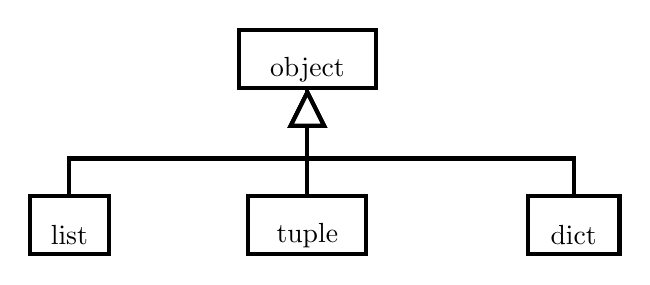
\begin{tikzpicture}
\pgftransformxscale{1.000000}
\pgftransformyscale{-1.000000}
\definecolor{dialinecolor}{rgb}{0.000000, 0.000000, 0.000000}
\pgfsetstrokecolor{dialinecolor}
\definecolor{dialinecolor}{rgb}{1.000000, 1.000000, 1.000000}
\pgfsetfillcolor{dialinecolor}
\pgfsetlinewidth{0.100000\du}
\pgfsetdash{}{0pt}
\definecolor{dialinecolor}{rgb}{1.000000, 1.000000, 1.000000}
\pgfsetfillcolor{dialinecolor}
\fill (24.038750\du,6.000000\du)--(24.038750\du,7.400000\du)--(27.336250\du,7.400000\du)--(27.336250\du,6.000000\du)--cycle;
\definecolor{dialinecolor}{rgb}{0.000000, 0.000000, 0.000000}
\pgfsetstrokecolor{dialinecolor}
\draw (24.038750\du,6.000000\du)--(24.038750\du,7.400000\du)--(27.336250\du,7.400000\du)--(27.336250\du,6.000000\du)--cycle;
% setfont left to latex
\definecolor{dialinecolor}{rgb}{0.000000, 0.000000, 0.000000}
\pgfsetstrokecolor{dialinecolor}
\node at (25.687500\du,6.950000\du){object};
\pgfsetlinewidth{0.100000\du}
\pgfsetdash{}{0pt}
\definecolor{dialinecolor}{rgb}{1.000000, 1.000000, 1.000000}
\pgfsetfillcolor{dialinecolor}
\fill (19.000000\du,10.000000\du)--(19.000000\du,11.400000\du)--(20.907500\du,11.400000\du)--(20.907500\du,10.000000\du)--cycle;
\definecolor{dialinecolor}{rgb}{0.000000, 0.000000, 0.000000}
\pgfsetstrokecolor{dialinecolor}
\draw (19.000000\du,10.000000\du)--(19.000000\du,11.400000\du)--(20.907500\du,11.400000\du)--(20.907500\du,10.000000\du)--cycle;
% setfont left to latex
\definecolor{dialinecolor}{rgb}{0.000000, 0.000000, 0.000000}
\pgfsetstrokecolor{dialinecolor}
\node at (19.953750\du,10.950000\du){list};
\pgfsetlinewidth{0.100000\du}
\pgfsetdash{}{0pt}
\definecolor{dialinecolor}{rgb}{1.000000, 1.000000, 1.000000}
\pgfsetfillcolor{dialinecolor}
\fill (24.266250\du,10.000000\du)--(24.266250\du,11.400000\du)--(27.108750\du,11.400000\du)--(27.108750\du,10.000000\du)--cycle;
\definecolor{dialinecolor}{rgb}{0.000000, 0.000000, 0.000000}
\pgfsetstrokecolor{dialinecolor}
\draw (24.266250\du,10.000000\du)--(24.266250\du,11.400000\du)--(27.108750\du,11.400000\du)--(27.108750\du,10.000000\du)--cycle;
% setfont left to latex
\definecolor{dialinecolor}{rgb}{0.000000, 0.000000, 0.000000}
\pgfsetstrokecolor{dialinecolor}
\node at (25.687500\du,10.950000\du){tuple};
\pgfsetlinewidth{0.100000\du}
\pgfsetdash{}{0pt}
\definecolor{dialinecolor}{rgb}{1.000000, 1.000000, 1.000000}
\pgfsetfillcolor{dialinecolor}
\fill (31.000000\du,10.000000\du)--(31.000000\du,11.400000\du)--(33.205000\du,11.400000\du)--(33.205000\du,10.000000\du)--cycle;
\definecolor{dialinecolor}{rgb}{0.000000, 0.000000, 0.000000}
\pgfsetstrokecolor{dialinecolor}
\draw (31.000000\du,10.000000\du)--(31.000000\du,11.400000\du)--(33.205000\du,11.400000\du)--(33.205000\du,10.000000\du)--cycle;
% setfont left to latex
\definecolor{dialinecolor}{rgb}{0.000000, 0.000000, 0.000000}
\pgfsetstrokecolor{dialinecolor}
\node at (32.102500\du,10.950000\du){dict};
\pgfsetlinewidth{0.100000\du}
\pgfsetdash{}{0pt}
\pgfsetmiterjoin
\pgfsetbuttcap
{
\definecolor{dialinecolor}{rgb}{0.000000, 0.000000, 0.000000}
\pgfsetfillcolor{dialinecolor}
% was here!!!
\definecolor{dialinecolor}{rgb}{0.000000, 0.000000, 0.000000}
\pgfsetstrokecolor{dialinecolor}
\draw (25.687500\du,7.400000\du)--(25.687500\du,9.100000\du)--(19.953750\du,9.100000\du)--(19.953750\du,10.000000\du);
}
\definecolor{dialinecolor}{rgb}{0.000000, 0.000000, 0.000000}
\pgfsetstrokecolor{dialinecolor}
\draw (25.687500\du,8.311803\du)--(25.687500\du,9.100000\du)--(19.953750\du,9.100000\du)--(19.953750\du,10.000000\du);
\pgfsetmiterjoin
\definecolor{dialinecolor}{rgb}{1.000000, 1.000000, 1.000000}
\pgfsetfillcolor{dialinecolor}
\fill (26.087500\du,8.311803\du)--(25.687500\du,7.511803\du)--(25.287500\du,8.311803\du)--cycle;
\pgfsetlinewidth{0.100000\du}
\pgfsetdash{}{0pt}
\pgfsetmiterjoin
\definecolor{dialinecolor}{rgb}{0.000000, 0.000000, 0.000000}
\pgfsetstrokecolor{dialinecolor}
\draw (26.087500\du,8.311803\du)--(25.687500\du,7.511803\du)--(25.287500\du,8.311803\du)--cycle;
% setfont left to latex
\pgfsetlinewidth{0.100000\du}
\pgfsetdash{}{0pt}
\pgfsetmiterjoin
\pgfsetbuttcap
{
\definecolor{dialinecolor}{rgb}{0.000000, 0.000000, 0.000000}
\pgfsetfillcolor{dialinecolor}
% was here!!!
\definecolor{dialinecolor}{rgb}{0.000000, 0.000000, 0.000000}
\pgfsetstrokecolor{dialinecolor}
\draw (25.687500\du,7.400000\du)--(25.687500\du,9.100000\du)--(32.102500\du,9.100000\du)--(32.102500\du,10.000000\du);
}
\definecolor{dialinecolor}{rgb}{0.000000, 0.000000, 0.000000}
\pgfsetstrokecolor{dialinecolor}
\draw (25.687500\du,8.311803\du)--(25.687500\du,9.100000\du)--(32.102500\du,9.100000\du)--(32.102500\du,10.000000\du);
\pgfsetmiterjoin
\definecolor{dialinecolor}{rgb}{1.000000, 1.000000, 1.000000}
\pgfsetfillcolor{dialinecolor}
\fill (26.087500\du,8.311803\du)--(25.687500\du,7.511803\du)--(25.287500\du,8.311803\du)--cycle;
\pgfsetlinewidth{0.100000\du}
\pgfsetdash{}{0pt}
\pgfsetmiterjoin
\definecolor{dialinecolor}{rgb}{0.000000, 0.000000, 0.000000}
\pgfsetstrokecolor{dialinecolor}
\draw (26.087500\du,8.311803\du)--(25.687500\du,7.511803\du)--(25.287500\du,8.311803\du)--cycle;
% setfont left to latex
\pgfsetlinewidth{0.100000\du}
\pgfsetdash{}{0pt}
\pgfsetmiterjoin
\pgfsetbuttcap
{
\definecolor{dialinecolor}{rgb}{0.000000, 0.000000, 0.000000}
\pgfsetfillcolor{dialinecolor}
% was here!!!
\definecolor{dialinecolor}{rgb}{0.000000, 0.000000, 0.000000}
\pgfsetstrokecolor{dialinecolor}
\draw (25.687500\du,7.400000\du)--(25.687500\du,8.250000\du)--(25.687500\du,9.950000\du)--(25.687500\du,10.000000\du);
}
\definecolor{dialinecolor}{rgb}{0.000000, 0.000000, 0.000000}
\pgfsetstrokecolor{dialinecolor}
\draw (25.687500\du,8.311803\du)--(25.687500\du,8.250000\du)--(25.687500\du,9.950000\du)--(25.687500\du,10.000000\du);
\pgfsetmiterjoin
\definecolor{dialinecolor}{rgb}{1.000000, 1.000000, 1.000000}
\pgfsetfillcolor{dialinecolor}
\fill (26.087500\du,8.311803\du)--(25.687500\du,7.511803\du)--(25.287500\du,8.311803\du)--cycle;
\pgfsetlinewidth{0.100000\du}
\pgfsetdash{}{0pt}
\pgfsetmiterjoin
\definecolor{dialinecolor}{rgb}{0.000000, 0.000000, 0.000000}
\pgfsetstrokecolor{dialinecolor}
\draw (26.087500\du,8.311803\du)--(25.687500\du,7.511803\du)--(25.287500\du,8.311803\du)--cycle;
% setfont left to latex
\end{tikzpicture}

    \end{center}
    \vspace{0.025\textheight}
    \texttt{boost::python::object} acts as the base class to all of these.
\end{frame}

%%%===========================================================================
\begin{frame}[fragile]{The almighty \pyobject}
    \onslide<1->
    \begin{itemize}
        \setlength{\itemsep}{0.05\textheight}
        \item base class for all Python objects
        \item provides access to virtually all functions of a type
    \end{itemize}
    \onslide<2->
    \vspace{0.1\textheight}
    \begin{minted}[fontsize=\small]{cpp}
void function(const object &o)
{
    o();                       //if object is callable
    o.attr("size");            //accessing an attribute
    o.attr("set_value")(2.13); //calling a method
    o[1] = "hell yeah";        //object list-like
    o["name"] = "Mustermann";  //object is map-like

    PyObject *ptr = o.ptr();   //access to Python pointer

}
    \end{minted}
\end{frame}
%%%===========================================================================
\begin{frame}[fragile]{Creating lists and tuples}
    Creating lists
    \begin{minted}{cpp}
list l;
l.append(1);
l.append("hello");
l.append(3.2);
std::cout<<len(l)<<std::endl;
l.insert(2,"world");
std::cout<<len(l)<<std::endl;
    \end{minted}
    
    \vspace{0.1\textheight}
    Creating tuples
    \begin{minted}{cpp}
tuple t = make_tuple(1,32,"hello");
    \end{minted}
\end{frame}

%%%===========================================================================
\begin{frame}[fragile]{Create instance on module level}
    \onslide<1->
    A class is just another object
    \begin{minted}[fontsize=\small]{cpp}
object class_sensor = class_<talk::sensor>("Sensor")
    .def(init<double>())
    .def("get_value",&talk::sensor::get_value)
    .def("set_value",&talk::sensor::set_value)
    .add_property("value",&talk::sensor::get_value,
                      &talk::sensor::set_value); 
    \end{minted}
    \onslide<2->
    \vspace{0.05\textheight} 
    \texttt{scope()} provides access to the current namespace
    \vspace{0.025\textheight}
    \begin{minted}[fontsize=\small]{cpp}
scope().attr("s2") = class_sensor(2.3);
    \end{minted}
    \vspace{0.05\textheight}
    \onslide<3->
    In Python we get
    \begin{minted}[fontsize=\small]{python}
import talk
print(talk.sensor.s2.value)
#output: 2.3
    \end{minted}
\end{frame}


